\documentclass[paper=a4, fontsize=12pt]{scrartcl} % A4 paper and 11pt font size

% \usepackage[T1]{fontenc} % use 8-bit encoding that has 256 glyphs
\usepackage{fourier}     % use the Adobe Utopia font for the document
                         % (comment this line to return to the LaTeX default)
%\usepackage{babel} % English language/hyphenation
\usepackage{amsmath,amsfonts,amsthm} % math packages
\usepackage{subeqnarray}

\usepackage{lipsum} % used for inserting dummy 'Lorem ipsum' text into the template
\usepackage{bold-extra}

\usepackage{gensymb}
\usepackage{listings}
\usepackage[utf8]{inputenc}
\usepackage{centernot}
\usepackage{mathrsfs}
\usepackage{amssymb}
\usepackage{physics}
\usepackage{verbatim}
\usepackage{fancyvrb}
\usepackage{biblatex}

% default fixed font does not support bold face
% \DeclareFixedFont{\ttb}{T1}{txtt}{bx}{n}{12} % for bold
% \DeclareFixedFont{\ttm}{T1}{txtt}{m}{n}{12}  % for normal

% custom colors
\usepackage{color}
\definecolor{deepblue}{rgb}{0,0,0.5}
\definecolor{deepred}{rgb}{0.6,0,0}
\definecolor{deepgreen}{rgb}{0,0.5,0}
\definecolor{lightblue}{rgb}{0.95,0.95,1}
\definecolor{lightgrey}{rgb}{0.6,0.6,0.6}
\usepackage{listings}

% use graphics packages
\usepackage{graphicx}
\usepackage{float}
\usepackage{tikz}
\usetikzlibrary{matrix}
\usetikzlibrary{calc}
\usetikzlibrary{patterns,fadings}

% python style for highlighting
\newcommand\pythonstyle{\lstset{
language=Python,
backgroundcolor=\color{lightblue},
basicstyle=\ttm,
otherkeywords={self,def},             % add keywords here
keywordstyle=\ttb\color{deepblue},
emph={while,for,if,elif,else,def,as,shape,conj,dot,copy,flatten,eye,zeros,ones,hstack,vstack,real,imag,conjugate,sin,cos,exp,append,insert,index,__main__}, % custom highlighting
%emphstyle=\ttb\color{deepred},     % custom highlighting style
emphstyle=\ttb\color{deepblue},     % custom highlighting style
stringstyle=\color{deepgreen},
commentstyle=\color{lightgrey},
frame=tb,                         % any extra options here
numbers=left,
showstringspaces=false            %
}}

% python environment
\lstnewenvironment{python}[1][]
{
\pythonstyle
\lstset{#1}
}
{}

% python for external files
\newcommand\pythonexternal[2][]{{
\pythonstyle
\lstinputlisting[#1]{#2}}}

% python for inline
\newcommand\pythoninline[1]{{\pythonstyle\lstinline!#1!}}


\usepackage{sectsty}        % allows customizing section commands
\allsectionsfont{\normalfont\scshape}      % make all sections centered
                                                      % the default font and small caps
\newcommand{\ssubsection}[1]{%
  \subsection[#1]{\raggedright\normalfont\itshape #1}}

\usepackage{fancyhdr}        % custom headers and footers
\pagestyle{fancyplain}       % makes all pages in the document conform to
                             % the custom headers and footers

% \renewcommand{\sectionmark}[1]{\markright{\thesection\ #1}}
\renewcommand{\sectionmark}[1]{\markboth{\thesection\ #1}{}}
\fancyhead[L]{\footnotesize\scshape\leftmark}
\fancyhead[R]{Page \thepage}


                             % the same way as the footers below
\fancyfoot[L]{\textit{Christopher R. McLeod}}              % empty left footer
\fancyfoot[C]{}              % empty center footer
\fancyfoot[R]{\textit{00947553}}      % page numbering for right footer
\renewcommand{\headrulewidth}{0.5pt}     % add header underlines
\renewcommand{\footrulewidth}{0.5pt}     % add footer underlines
\setlength{\headheight}{13.6pt}        % customize the height of the header



\numberwithin{equation}{section}       % number equations within sections
                                       % (i.e. 1.1, 1.2, 2.1, 2.2 instead of 1, 2, 3, 4)
\numberwithin{figure}{section}         % number figures within sections
                                       % (i.e. 1.1, 1.2, 2.1, 2.2 instead of 1, 2, 3, 4)
\numberwithin{table}{section}          % number tables within sections
                                       % (i.e. 1.1, 1.2, 2.1, 2.2 instead of 1, 2, 3, 4)

\setlength\parindent{24pt}         % removes all indentation from paragraphs
                                  % comment this line for an assignment with lots of text


% \usepackage[T1]{fontenc}
\usepackage{enumerate}

% \usepackage[tocflat]{tocstyle}
\allowdisplaybreaks
\makeatletter
\setcounter{tocdepth}{4}
% \renewcommand\tableofcontents{%
%   \null\hfill\textsc{\Large\contentsname}\hfill\null\par
%   \vspace{1cm}
%   \@mkboth{\MakeUppercase\contentsname}{\MakeUppercase\contentsname}%
%   \@starttoc{toc}%
% }
% \renewcommand*\l@section{\ifnum\c@tocdepth>\z@\vskip 6pt plus 1pt minus 1pt \fi
%                          \@dottedtocline{1}{1.5em}{2.3em}}
% \renewcommand{\@pnumwidth}{1.75em}
% \renewcommand{\@tocrmarg}{2.75em}
\makeatother
\usepackage{empheq}


%--------------------------
%	TITLE SECTION
%--------------------------
\renewcommand*\contentsname{Summary}

\newcommand{\horrule}[1]{\rule{\linewidth}{#1}} % create horizontal rule command
                                                % with 1 argument of height


\renewcommand*\footnoterule{}


\title{
\normalfont \normalsize
\textsc{Imperial College London, Department of Mathematics} \\ [25pt]
\horrule{0.5pt} \\[0.4cm]                      % thin top horizontal rule
\huge M4N9 Project 2: \\ An Example of Matrix Structure 
Exploitation in Solving Linear Systems \\           % the assignment title
\horrule{2pt} \\[0.5cm]                        % thick bottom horizontal rule
}


\author{Christopher McLeod}
\date{\normalsize\ November 27, 2017}

\begin{document}
%\ttfamily
%\fontseries{b}\selectfont

\titlepage
\maketitle
\begin{center}
  
\includegraphics[width=100pt]{crest.png} \\

  \vfill
  \vspace{4.2cm}
  \textbf{Abstract} \\
In this project, the aim is to improve the complexity and run-time of an algorithm which solves a linear system of equations. The focus is on accomplishing this goal by exploiting certain properties and structure of the system. The system in question is determined from a model of a problem from fluid dynamics.  \\
\end{center}
\thispagestyle{empty}

%-----------------------------------------------------------------------
% contents page
%-----------------------------------------------------------------------

\thispagestyle{empty}
\tableofcontents
\newpage

%-----------------------------------------------------------------------
% Rest of Paper
%-----------------------------------------------------------------------

\section*{\centerline{Foreword}}

In the interest of making this paper as concise as possible, in general functions and scripts have been excluded from the final write-up. What is included is a description of the algorithms and programs, in terms of what function they perform. For the implementation,the code is provided alongside this paper with detailed comments.\\

\addcontentsline{toc}{section}{Introduction: Statement of the Problem}
\section*{Introduction: Statement of the Problem}

The problem used to explore the effects of matrix exploitation is one in fluid dynamics. In this problem, We envisage $N$ spherical particles equispaced along a horizontally on a planar surface. When moving through the fluid, the forces on the particles are drag, which opposes the motion of the particle, and interaction forces from the disturbances caused by other particles moving through the fluid. 

\indent The motion is assumed to be slow enough that the drag is linear, so we can describe the problem with a linear system 

$$ MF = V $$
Or, more explicitly 
$$
  \begin{bmatrix}
     M_{11} & M_{12} & \, &\cdots & \, & M_{1N} \\
     M_{21} & M_{22}  & \, &\cdots & \, & M_{2N} \\
     \vdots & \vdots & \, & \ddots & \,  & \vdots \\
     M_{N1} & M_{N2} & \,  & \cdots & \, & M_{NN}
  \end{bmatrix}
  \begin{bmatrix}
    F_1 \\
    F_2 \\
    \vdots \\
    F_N
  \end{bmatrix}
  =
  \begin{bmatrix}
    V_1 \\
    V_2  \\
    \vdots \\
    V_N 
  \end{bmatrix}
  \\
$$

\noindent where $F_i$ and $V_i$ correspond to the force and velocity (respectively) of the $i^{th}$ particle, $1 \leq i \leq N$. They are both $2\times1$ vectors with each entry corresponding to the force/velocity of the particle in each planar direction, e.g 

$$ V_i = 
\begin{bmatrix}
V_{i_{x}} \\
V_{i_{y}} 
\end{bmatrix} $$

\noindent where we are $V_{i_{x}}$ describes the velocity in the $x$-direction of the $x-y$ plane.\\

\noindent $M$ here is the matrix of $M_{ij}$ which are $2\times2$ matrices that describe the contribution to the velocity $i$ by the force on particle $j$. These matrices are calculated using the \textit{Rotne-Prager-Yamakawa} (or \textit{RPY}) tensor, which depends on the distance of particle $i$ to $j$. 

\noindent We can describe the individual $M_{ij}$ as 

$$ M_{ii} = 
\begin{pmatrix}
c^d_{i_{x}} & 0 \\
0 & c^d_{i_{y}}
\end{pmatrix}
$$

\noindent where $c^d$ is the drag coefficient and $c^d_{i_{x}}$ is the drag coefficient for particle $i$ moving in the $x$-direction. And if $i \neq j$ 

$$ M_{ij} = 
\begin{pmatrix}
 \sigma^I_{(i\rightarrow j)_{x}} & 0 \\
0 & \sigma^I_{(i\rightarrow j)_{y}}
\end{pmatrix}
$$

\noindent where $\sigma^I_{(i\rightarrow j)_{x}}$ is the coefficient describing the interaction of particle $i$ on $j$.  

\indent They are set up this way because of course a particle causing disturbances in the fluid which have an effect on itself is is exactly what we call drag. The zeros on the off-diagonal arise from the planarity of the motion, e.g forces in the y-direction should not contribute to motion in the x-direction. \\

\noindent We now set about using the above the matrices above to solve the system $MF = V$ for $F$. 


\section{Part 1: The Unabridged System}

We set up the above problem for uniform motion in the y-direction 

$$ V_i = 
\begin{bmatrix}
0 \\ 
1
\end{bmatrix} $$

\noindent The function \texttt{Msetup} creates the $M$ matrix by making calls to \texttt{RPY2D} to calculate the interaction/drag coefficients. 
The system is then solved for $F$ by using \texttt{parpivgelim} to give $L$,$U$ and $P$ such that 

$$ PM = LU$$ 

\noindent where P is a $2N\times 2N$ permutation matrix such that $L$ and $U$ are lower/upper triangular respectively. Then, using the fact that $P$ is orthogonal we get 

$$ MF = V \iff PMF = P \iff LUF = PV$$

\noindent From here we simply use forward substitution (carried out by the function \texttt{fwdsub}) to solve the system $Lz = PV$ for $z = UF$ and subsequently use backward substitution (via \texttt{backsub}) to solve $UF = z$ for $F$. This is done by the function \texttt{Force}, which takes the values $b$ (the parameter giving spacing between the particles) and $N$, sets up and solves the above problem in the described way. 

\subsection{The Solution}
The function \texttt{plotFnorm} makes calls to \texttt{Force} with input $(b,N)$ for combinations of $b$ and $N$, such that $b\in\{2,4,10\}$ and $N\in\{100,200,400\}$. For each pair the solution $F$ (the second function output of \texttt{Force}) is calculated and its norm, $\norm{F}_2$ is stored. This produces the table \ref{table:1}.

\begin{table}
\begin{center}
  \begin{tabular}{ c||c|c|c }
           & N=100 &    N=200 &    N=400 \\
	\hline 

    b=2  &   45.055  &  73.557&    116.03 \\
    b=4    & 56.482 &   94.408 &   154.24 \\
    b=10  &  71.752  &  122.19   & 205.76
  \end{tabular}
\end{center}
\caption{$\norm{F}_2$ for varying $b$ and $N$}
\label{table:1}
\end{table}

\noindent The Force itself is also stored by \texttt{plotFnorm} and is plotted as a function of $x_i/x_N$ (to scale the results) on 3 graphs, which plot the Force for fixed $N$ and varying $b$, shown in plots \ref{fig:Fplot1}, \ref{fig:Fplot2} and \ref{fig:Fplot3}. 

\begin{figure}[h!]
  \centering
  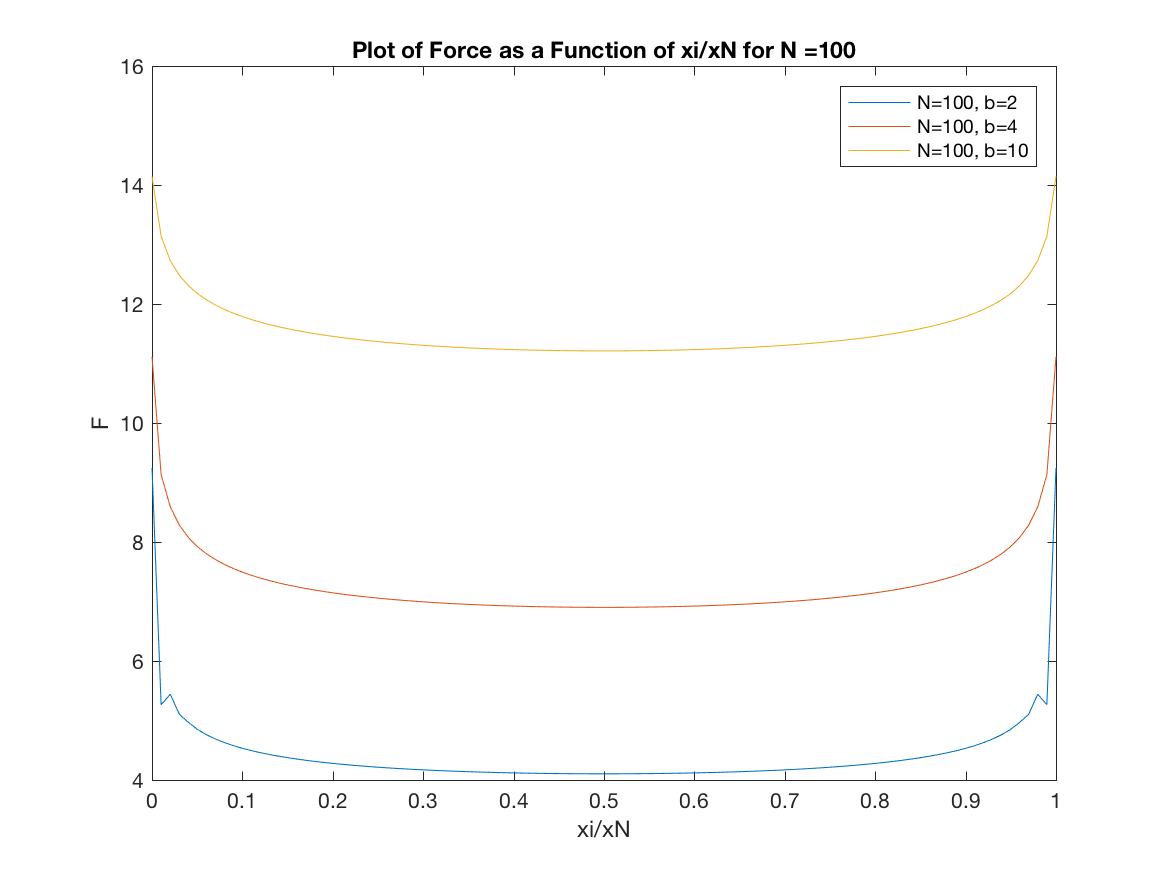
\includegraphics[width=0.8\textwidth]{Plot_of_Force_N100.png}
  \caption{plot of Force as a function of $x_i/x_N$ for $N=100$}
  \label{fig:Fplot1}
\end{figure}

\begin{figure}[h!]
  \centering
  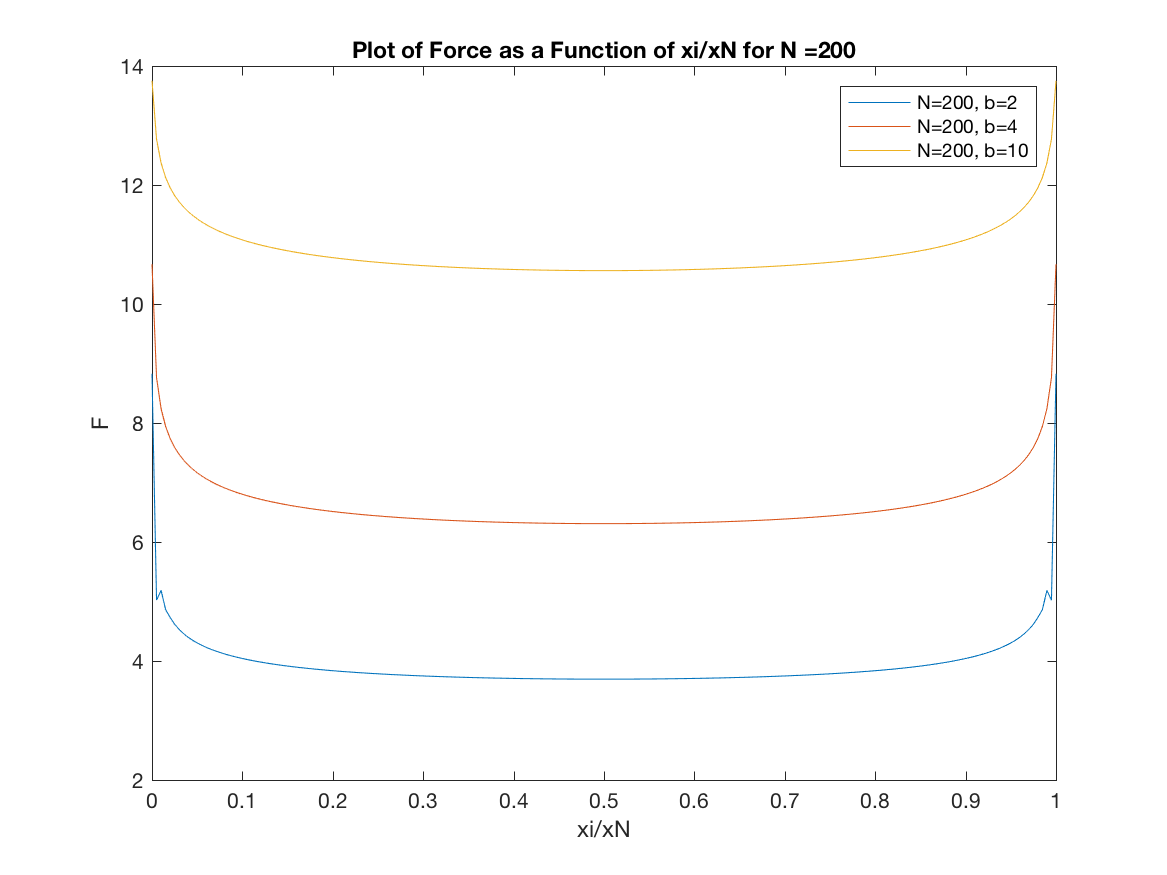
\includegraphics[width=0.8\textwidth]{Plot_of_Force_N200.png}
  \caption{plot of Force as a function of $x_i/x_N$ for $N=200$}
  \label{fig:Fplot2}
\end{figure}

\begin{figure}[h!]
  \centering
  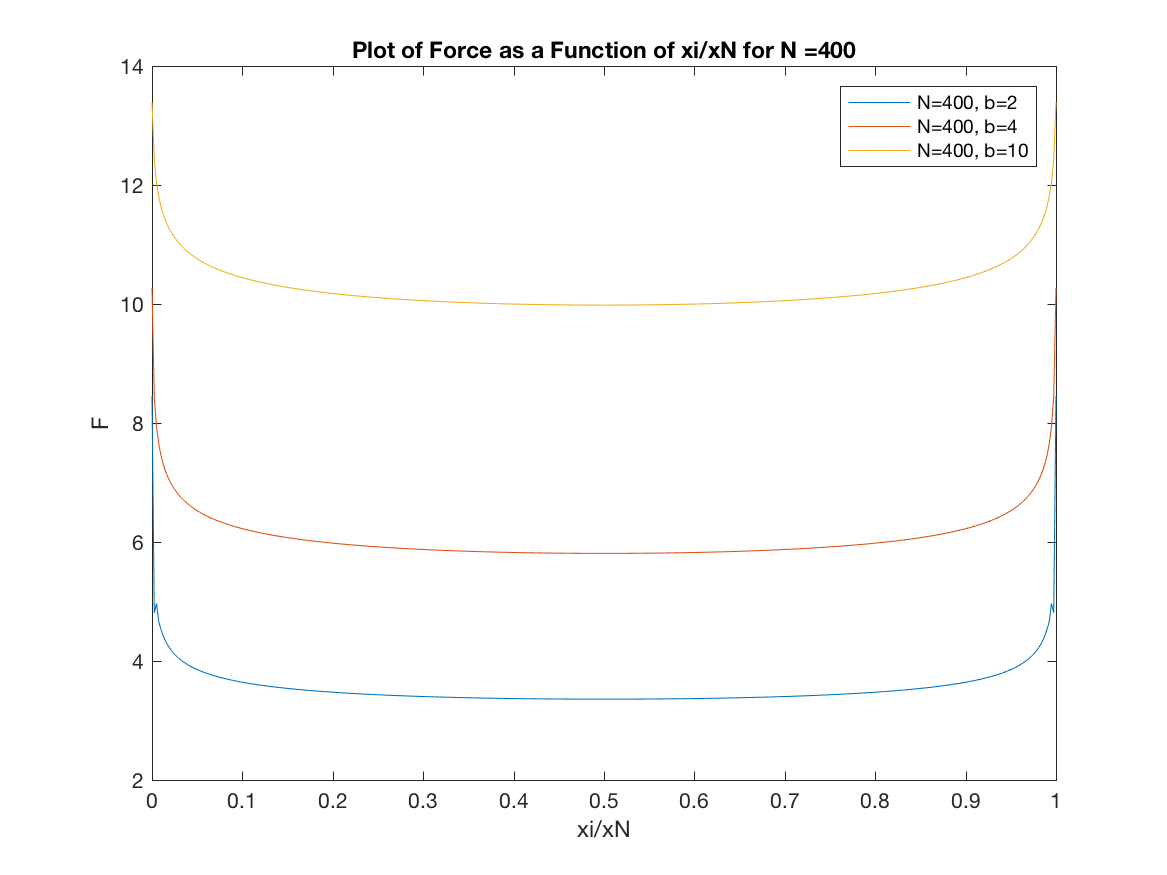
\includegraphics[width=0.8\textwidth]{Plot_of_Force_N400.png}
  \caption{plot of Force as a function of $x_i/x_N$ for $N=400$}
  \label{fig:Fplot3}
\end{figure}
\newpage 
\noindent The three graphs look very similar, which indicates that the spacing parameter has a much greater effect on the distribution of the force across the particles than the number of them. While we can see the troughs of the forces graphs for any $N$ are slightly lower for increasing $N$, the most discernible difference arises from decreasing $N$. 

\indent Looking at the table seems to tell a different story however. The norm of the force vector generally increases more with $N$ than it does with $b$ and would suggest that $N$ has more of an effect on the size of the force than the distance between them. \\

\noindent In conclusion, we can say that the size of the force in the system is most affected by the number of particles, but generally the force felt by particle $i$ is most affected by the spacing between the particles. 


\newpage 
\subsection{The Complexity of the Algorithm} 
We have seen in lectures that the partial-pivot LU-decomposition has complexity $O(N^3)$ (i.e. computes $O(N^3)$ flops) if the matrix on which it is performed has dimensions $N\times N3$. This is investigated below. 

\indent The function \texttt{Forcetime} makes 5 calls to Force. It sets $b=4$ and varies $N$ on each loop to take on  the values $100, 200, 400, 800, 1600$. \texttt{Force} returns, as it's first function output, the time taken to decompose M and solve the system for $F$, which is stored by \texttt{Forcetime} in $5\times 1$ vector, corresponding to the values of $N$. A log-log plot of the run-time of \texttt{Force(4,N}) against $N$ gives plot \ref{fig:Forcelog}.

\begin{figure}[h!]
  \centering
  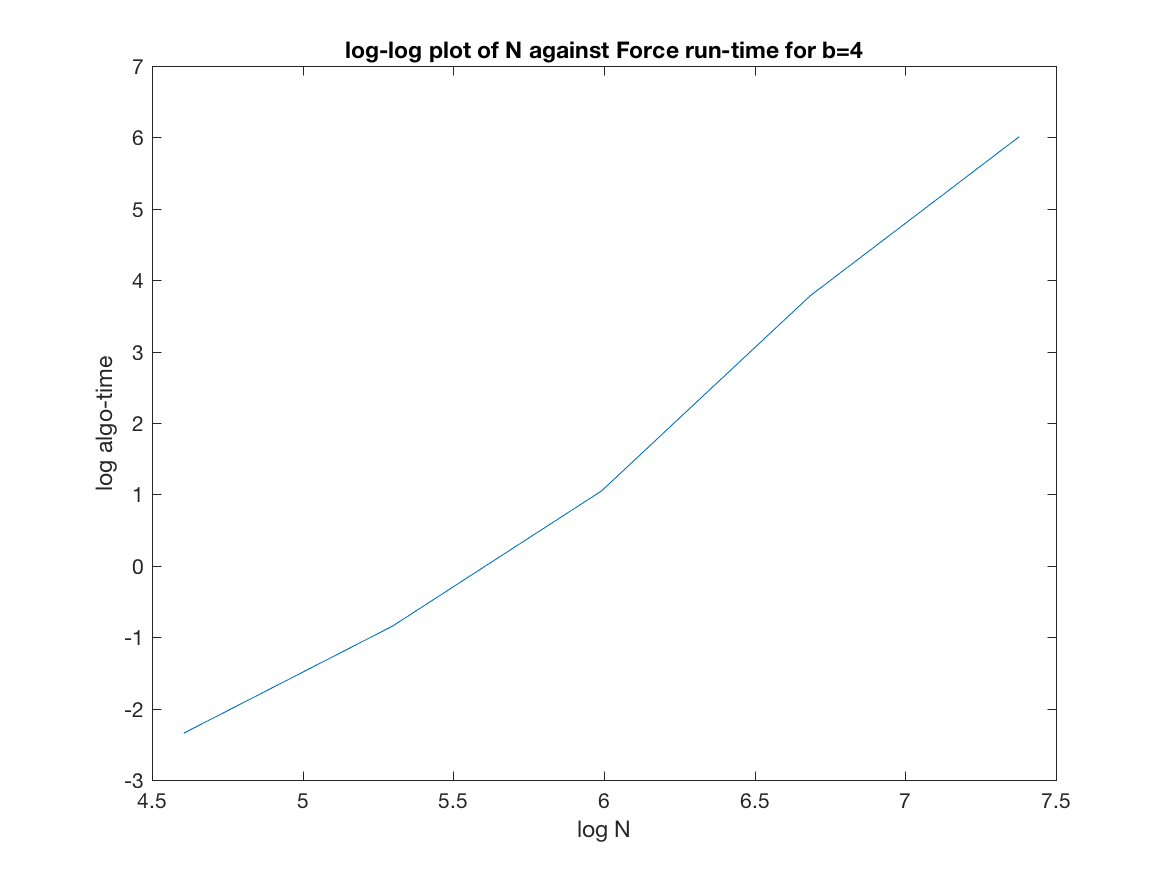
\includegraphics[width=0.8\textwidth]{log-log_plot_Force.png}
  \caption{log-log plot of \texttt{Force(4,N)} run-time against $N$} 
  \label{fig:Forcelog}
\end{figure}

\noindent The second function output of \texttt{Forcetime} is \texttt{grad}. This value is given by taking the gradient of a linear regression performed on the log-log graph using \texttt{polyfit} as a way of approximating the log-complexity of the algorithm. Calling this output gives (after some time)
\begin{verbatim}
>> [~,grad] = Forcetime()

grad =

    3.0992
\end{verbatim}
Which looks roughly accurate, given the random deviation inherent in timing any algorithm. 

\subsection{Stability of the Algorithm} 
We have seen in lectures that the LU-decomposition with partial pivoting algorithm is backwards stable. That is, for the growth factor 

$$ \rho = \frac{\max_{i,j} \abs{u_{ij}} } {\max_{i,j} \abs{M_{ij}}} $$

\noindent where $M_{ij}$ are the scalar entries in $M$ and $U_{ij}$ are the scalar entries of the upper triangular matrix of the LU decomposition of M, we are assured that LU-decomposition produces $\widetilde{L},\widetilde{U},\widetilde{P}$ such that 

$$ \widetilde{L}\widetilde{U} = \widetilde{P} M + \delta M \quad \textit{such that} \quad \frac{\norm{\delta M}}{\norm{ M}} = O(\rho \epsilon) $$

\noindent where $\epsilon$ is machine epsilon. The above is of course the definition of backward stability.\\

\noindent The function \texttt{backLU} fixes $b=4$ and plots $\norm{\delta M}/\norm{ M}$ and $\norm{\delta M}/\rho\norm{M}$ for $N\in \{100,200,400\}$. The plot \ref{fig:residualplot} displays the residual against value of $N$

\begin{figure}[h!]
  \centering
  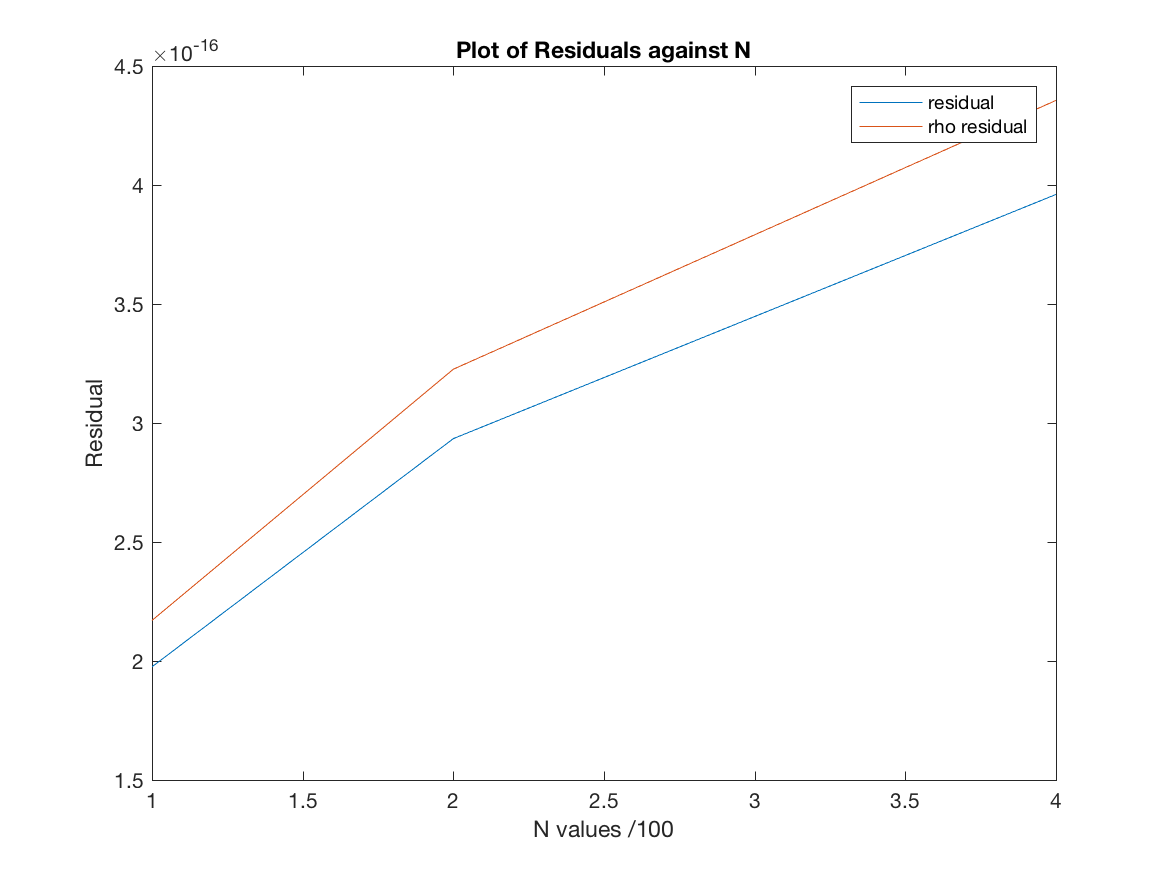
\includegraphics[width=0.8\textwidth]{residual_plot.png}
  \caption{Plot of Residual Error against $N$} 
  \label{fig:residualplot}
\end{figure}

\noindent The graph does show increasing residual error, but also that $\rho$ sticks around 1 and both the residual and adjusted residual are below machine error. One could say this provides numerical evidence for the residual being  $O(\rho\epsilon)$.


\section{Part 2: Reducing The Problem}
The LU-decomposition with partial pivoting takes $\sim \frac{2}{3}m^3 + O(m^2)$ FLOPs to execute on an $m\times m$ matrix. In the above section, when $N=1600$ this means the algorithm does $\sim O(10^{10})$ FLOPs in decomposing $M$, and the run-time in this case was around $450s$ \textit{(}$\sim 8$ \textit{min)}, which is a very long time to wait. 

\indent This can be improved by permuting the system to solve the problem more concisely, this is apparent simply because half of the matrix $M$ has the value $0$ and these $0s$ occur regularly. 
\subsection{Analysing the Matrix Structure}
Experimenting by varying the parameters $b$ and $N$ in the system shows that the structure is dependent on $N$ and the values depend on $b$. This is logical of course because the spacing parameter affects the distance between particles, which is exactly how the RPY-tensor calculates the interaction/drag coefficients. As discussed in the introduction, the $M_{ij}$ (that is, the $2\times 2$ matrix entries of $M$) have structure 
$$M_{ij} = 
\begin{pmatrix}
 \sigma^I_{(i\rightarrow j)_{x}} + \delta_{ij}(c^d_{i_{x}} - \sigma^I_{(i\rightarrow j)_{x}}) & 0 \\
0 &  \sigma^I_{(i\rightarrow j)_{y}} + \delta_{ij}(c^d_{i_{y}} - \sigma^I_{(i\rightarrow j)_{y}})
\end{pmatrix}
$$
\noindent where $\delta_{ij}$ is the Kronecker-delta function. This gives $M$ the general structure
$$M = 
\begin{bmatrix}
\left(\begin{matrix}
	c^d_{1_{x}} & 0 \\
	0 & c^d_{1_{y}}
\end{matrix} \right) & \left(\begin{matrix}
				 \sigma^I_{(1\rightarrow 2)_{x}} & 0 \\
				 0 & \sigma^I_{(1\rightarrow 2)_{y}}
				 \end{matrix}\right) & \, &\cdots & \, & \left(\begin{matrix}
									 \sigma^I_{(1\rightarrow N)_{x}} & 0 \\
									 0 & \sigma^I_{(1\rightarrow N)_{y}}
									 \end{matrix}\right) \\
\left(\begin{matrix}
 \sigma^I_{(2\rightarrow 1)_{x}} & 0 \\
	0 & \sigma^I_{(2\rightarrow 1)_{y}}
\end{matrix}\right) & \left(\begin{matrix}
				 c^d_{2_{x}} & 0 \\
				 0 & c^d_{2_{y}}
				\end{matrix}\right)  & \, &\cdots & \, & \left(\begin{matrix}
													 \sigma^I_{(2\rightarrow N)_{x}} & 0 \\
													0 & \sigma^I_{(2\rightarrow N)_{y}}
												   \end{matrix}\right) \\
 \vdots & \vdots & \, & \ddots & \,  & \vdots \\
 \left(\begin{matrix}
 \sigma^I_{(N\rightarrow 1)_{x}} & 0 \\
 0 & \sigma^I_{(N\rightarrow 1)_{y}}
 \end{matrix}\right) & \left(\begin{matrix}
				 \sigma^I_{(N\rightarrow 2)_{x}} & 0 \\
				 0 & \sigma^I_{(N\rightarrow 2)_{y}}
				\end{matrix}\right) & \,  & \cdots & \, & \left(\begin{matrix}
														c^d_{N_{x}} & 0 \\
														0 & c^d_{N_{y}}
													\end{matrix}\right)
\end{bmatrix}
$$
\noindent This can be re-written for clarity as
$$M = 
\begin{bmatrix}
c^d_{1_{x}} & 0 		  & \, & \cdots & \, &   \sigma^I_{(1\rightarrow N)_{x}}	&		 0 \\
0		    & c^d_{2_{x}} & \, &\cdots & \, & 0 &   \sigma^I_{(2\rightarrow N)_{y}} \\
 \vdots & \vdots & \, & \ddots & \,  & \vdots \\
\sigma^I_{(N\rightarrow 1)_{x}} & 0 & \, &\cdots & \, & c^d_{N_{x} & 0 \\
0 & \sigma^I_{(N\rightarrow 2)_{y}} & \, & \cdots & \, & 0 & c^d_{N_{y}}
\end{bmatrix}
$$

\noindent The interaction and drag terms are calculated by the RPY tensor in \texttt{RPY2D} which depend only on $b$. As $b$ increases, the distance between the particles increases and so the value of the interaction forces $\sigma^I_{(i\rightarrow j)_{y}}$ decreases. Drag remains the same as $b$ changes however: as the distance is zero and the assumption is made that the drag contributes equally, regardless of how spaced the particles are.

\noindent Observations made by experimenting with \texttt{RPY2D} show that in fact the matrix is Toeplitz and symmetric. The former means we expect drag to contributes to oppose the motion, regardless of which direction the motion is (i.e moving left, up or at a $45\degree$ angle will give the same drag coefficient) for all particles. The latter means for all particles $i$ and $j$, the contribution to the velocity of particle $i$ by the force on particle $j$ is equal to that of $j$ on $i$ - i.e $\sigma^I_{(i\rightarrow j)} = \sigma^I_{(j\rightarrow i)}$. Another thing that is apparent is that contribution to the velocity of the interaction terms for any two particles is equal in the $x$ and $y$ direction. So in total, we know the following about the matrix $M$ for any $i$ and $j$ 
\begin{equation}
 c^d_{i_{x}} = c^d_{j_{y}}
\end{equation}

\begin{equation}
\sigma^I_{(i\rightarrow j)_{x}} = \sigma^I_{(j\rightarrow i)_{x}} = \sigma^I_{(j\rightarrow i)_{y}}
\end{equation}

\subsection{Permuting to Reduce} 
The information about the position of the zeros in $M$ and the structure of $M_{ij}$ alone is enough to see that it makes sense to permute $M$ to exploit these zeros. A zero occurs at $m_{ij}$ (the scalar entries of $M$) whenever the sum its indices $i+j$ is odd. For example, $m_{11}$ is non-zero because the $1+1=2$ but  $m_{21}, m_{41},m_{16}$ are all zero in $M$. \\

\noindent The aim here is to bunch the non-zero terms together into smaller square matrices. The zeros of M alternate along the rows and columns, so we seek a permutation matrix which moves the zeros of rows $2,4,6,\dots,2N$ to the bottom of $M$, while the non-zero terms in rows $1,3,5,\dots,2N-1$ move down. Then by right multiplying the transpose of the matrix, the zeros in the columns of $2,4,6$ move right in $M$ while the non-zero terms in columns $1,3,5,\dots,2N-1$ move left.\footnote{while the discussion is of zeros of the odd/even rows/columns moving, everything else in the specified row/column is moving with it, only this way the important moves are documented.} 

\indent The result of these transformations is 

$$ 
PMP^T = 
\begin{bmatrix}
M1 & 0 \\ 
0 & M2 
\end{bmatrix}
$$

\noindent where P is some permutation matrix, 0 denotes the $N\times N$ matrix of zeros and M1 and M2 contain all the interaction terms of $M$. Here is an example of the above reduction carried out for the case where we have $N=2$ particles. 

\begin{align*}
PMP^T &= 
	\left[ \begin{matrix}
	1 & 0 & 0 & 0 \\
	0 & 0 & 1 & 0 \\ 
	0 & 1 & 0 & 0 \\ 
	0 & 0 & 0 & 1 
	\end{matrix} \right] 
	\left[ \begin{matrix}
	c^d_{1_{x}} & 0 & \sigma^I_{(1\rightarrow 2)_{x}} & 0 \\
	0 			& c^d_{1_{y}} & 0 & \sigma^I_{(1\rightarrow 2)_{y}} \\
	\sigma^I_{(2\rightarrow 1)_{x}} & 0 & c^d_{2_{x}} & 0 \\
	0 & \sigma^I_{(2\rightarrow 1)_{y}} & 0 & c^d_{2_{y}} 
	\end{matrix} \right]
	\left[ \begin{matrix}
	1 & 0 & 0 & 0 \\
	0 & 0 & 1 & 0 \\ 
	0 & 1 & 0 & 0 \\ 
	0 & 0 & 0 & 1 
	\end{matrix} \right]
\\
&=
	\left[ \begin{matrix}
	c^d_{1_{x}} & 0 & \sigma^I_{(1\rightarrow 2)_{x}} & 0 \\
	\sigma^I_{(2\rightarrow 1)_{x}} & 0 & c^d_{2_{x}} & 0 \\
	0 & c^d_{1_{y}} & 0 & \sigma^I_{(1\rightarrow 2)_{y}} \\
	0 & \sigma^I_{(2\rightarrow 1)_{y}} & 0 & c^d_{2_{y}} 
	\end{matrix} \right]
	\left[ \begin{matrix}
	1 & 0 & 0 & 0 \\
	0 & 0 & 1 & 0 \\ 
	0 & 1 & 0 & 0 \\ 
	0 & 0 & 0 & 1 
	\end{matrix} \right]
\\
&= \quad \quad \quad
	\left[ \begin{matrix}
	c^d_{1_{x}} & \sigma^I_{(1\rightarrow 2)_{x}} & 0 & 0 \\
	\sigma^I_{(2\rightarrow 1)_{x}} & c^d_{2_{x}} & 0 & 0 \\
	0 & 0 & c^d_{1_{y}} & \sigma^I_{(1\rightarrow 2)_{y}} \\
	0 & 0 &  \sigma^I_{(2\rightarrow 1)_{y}}  & c^d_{2_{y}} 
	\end{matrix} \right]
\\
\end{align*} 
\noindent The permutation matrix here is it's own transpose. In the $N=3$ case, the permutation matrix is 

$$P_3 = 
\begin{bmatrix}
1 & 0 & 0 & 0 & 0 & 0 \\ 
0 & 0 & 1 & 0 & 0 & 0 \\ 
0 & 0 & 0 & 0 & 1 & 0 \\
0 & 1 & 0 & 0 & 0 & 0 \\ 
0 & 0 & 0 & 1 & 0 & 0 \\ 
0 & 0 & 0 & 0 & 0 & 1 
\end{bmatrix}
$$

\\


\noindent Since the zeros in the rows alternate, we can build the matrix for any $N$ by the following algorithm 

\begin{enumerate}
\item Set row 1 equal to $\widehat{e_1}^T$ (the first of the canonical basis vectors of $R^{2N}$) 
\item Move down a row, set it equal to the above row with the 1-entry displaced 2 columns to the right
\item Repeat step 2 until every row of the matrix has been filled
\end{enumerate}

\noindent Note that this actually determines the last row of $P$ as 1. The 1-entry moves $N-1$ times in between 1 and the $N^{th}$ where its column is $1 + 2(N-1) = 2N-1$. Its column in row $N+1$ is 2 and it jumps another $N-1$ times to column $2 + 2(N-1) = 2N$. So the general permutation matrix looks like 

$$ P_N = 
  \begin{bmatrix}
     1 & 0 & 0  & \, &\cdots & \, & 0 & 0 & 0  \\
     0 & 0 & 1  & \, &\cdots & \, & 0 & 0 & 0 \\
     \vdots & \vdots & \vdots & \, & \ddots & \, & \vdots & \vdots & \vdots \\
     0 & 0 & 0 & \, &\cdots & \, & 0 & 1 & 0 \\ 
	 0 & 1 & 0 & \, &\cdots & \, & 0 & 0 & 0 \\	
     \vdots & \vdots & \vdots & \, & \ddots & \, & \vdots & \vdots & \vdots \\
	 0 & 0 & 0  & \, & \cdots & \, & 0 & 0 & 1   
  \end{bmatrix}
$$

\noindent From the set-up of $M$ as in 2.1 and the above description, we can see that the permutation matrix switches the rows and columns such that the interactions in the two blocks $M1$ and $M2$ correspond to the interactions in the $x$ and $y$ direction respectively. 
\\ 
\noindent The system can be augmented to include this result in the following way 
\begin{align*}
MF = V &\iff PMF = PV \\
	   &\iff (PMP^T)(PF) = PV 
\end{align*}
\noindent since $P$ is orthogonal as a permutation matrix. $P$ acts on $F$ and $V$ in the same way so that the $x$ and $y$ components of the force/velocity are permuted into the top/bottom half of the vector. This is obvious as the top half of $P$ takes the first and then every second entry proceeding - exactly the $x$-components of the force/velocity - and moves them to the top (in order). Similarly the bottom half of $P$ puts the $y$-components in the bottom of the vector. So now we have two smaller systems \\ 
Let $V_x = (PV)_{1:N}$, $V_y = (PV)_{N+1:2N}$, $F_x = (PF)_{1:N}$, $F_y = (PF)_{N+1:2N}$ then

\begin{empheq}[left = \empheqlbrace]{align*}
M1F_x &= V_x \\
M2F_y &= V_y 
\end{empheq}


\noindent So we have reduced a $2N\times 2N$ system to two $N\times N$ systems. We can observe from the above that the way the permutation matrix works means we never have to actually multiply by $P$. This can all be done by array slicing the original system. For example, if we want $F_x$, we simply perform the array slice 

\begin{verbatim}
	F_x = F(1:2:2*N)
\end{verbatim}


\noindent which grabs every second term of $F$ starting from the first term of $F$. We can also do the same for $M$, given its structure as describes in part 2.1

\begin{verbatim}
	M1 = M(1:2:2*N, 1:2:2*N)
\end{verbatim}


\section{Part 3: Exploiting the Structure}
Considering the system as we did in part 1, where $V_i = \left[0, 1\right]^T$, i.e all motion is in the $y$-plane, we can use the results in Part 2 to speed the solution. 

\noindent Using the notation as in Part 2, we get $V_x = 0$ which implies $F_x = 0$ so instead of solving the original $2N\times 2N$ system, we can settle for solving the $N\times N$ system 
$$
M2F_y = V_y
$$

\subsection{Speeding up the Reduced System}
More than this, we can use the standard LU-decomposition in place of the LU-decomposition with partial pivoting in solving the system. The latter does $O(m^2)$ FLOPs more for the LU-decomposition of an $m\times m$ matrix than the former. 

\indent  This is because the RPY-tensor calculates the drag to be the largest force on the particle. Due to it's definition in our system, the $c^d = 1/(6\pi)$ for any particle in the x or y contribution. The largest interaction forces (where $r_{ij} \leq 2a$ but $r_{ij} \neq 0 $) are strictly less than this value, since if we let $X_i,X_j$ be of minimal distance $b$, then 
$$
\qquad - \frac{9}{32a}bI + \frac{3b}{32a}\frac{(X_i - X_j)(X_i - X_j)^T}{b^2} \\
= -\frac{9}{32a}bI + \frac{3}{32a}b      \begin{pmatrix}
											0 & 0 \\ 
											0 & 1 
										\end{pmatrix} \\
$$
$$
= -\frac{1}{32a}\begin{pmatrix} 
				9 & 0 \\ 
				0 & 6		
			  \end{pmatrix} b
$$
and so the matrix of contribution to the velocity of particle $i$ by particle $j$ \textit{always} has value less than $c^d$ in our system. \\

\noindent In light of these reductions, the function \texttt{parpivgelim} is replaced by \texttt{gelim} which performs the standard LU-decomposition without pivoting. It is used on the second reduced system to find the only unknown $F_y$. After the standard LU-decomposition is computed, the solution is found by forward then backward substitution as before. 

\indent To see the what effect this has on run time, $b=4$ is fixed as in Part 1.2 and similarly, the run-time is measured and plotted on a log-log graph (via the function \texttt{fastForce}) to produce plot \ref{fig:fastForce}.

\begin{figure}[h!]
  \centering
  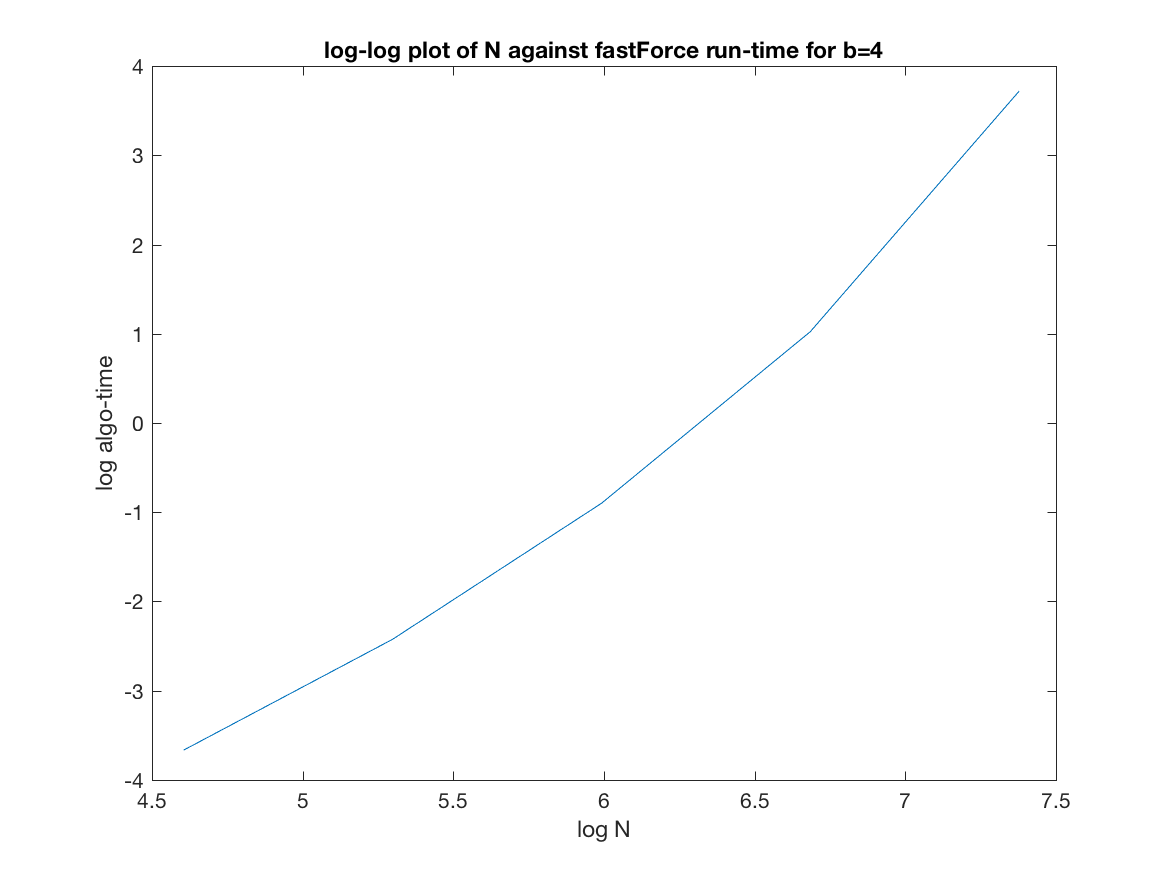
\includegraphics[width=0.8\textwidth]{log-log_plot_fastForce.png}
  \caption{log-log plot of \texttt{fastForce} against $N$}
  \label{fig:fastForce}
\end{figure}

\noindent By taking advantage of the decomposability of $M$ into $M2$ to halve the size of the system, and by realising the largest terms of $M2$ are on the diagonal to eliminate the need for pivoting, there has been a significant speed-up in run-time. Comparing the graphs for the largest system ($N=1600$) suggests the run-time has been reduced from $\sim\exp(6) $  to $\sim\exp(4)$ which is a reduction of $\sim 350s$, from an original run time of $\sim 400s$! This is an improvement of $\sim \% 700 $ in the most extreme case. 

\noindent The comprehensive speed-up ratios can be seen in table \ref{table:3}. 

\subsection{Taking Advantage of the Structure}
In Part 2.1 we identified that $M$ is Toeplitz and symmetric. Considering the effect of the permutation and its result in Part 2.2, we can see that $M1$ and $M2$ also exhibit the same structure. This makes $M2$ positive-definite, and so it immediately becomes possible to reduce the decomposition time to at least Cholesky-like time ($m^3/3$ FLOPs), but actually the Toeplitz structure means we can decompose $M2$ even faster. \\

\noindent The most efficient solution to solve symmetric positive definite Toeplitz systems (in general) is via the Levinson algorithm given in Golub and Van Loan. The entire solve can be done in just $O(m^2)$ FLOPs for an $m\times m$ matrix$^{[1]}$. This is an enormous difference, given that in the above part, we were doing LU-decomposition, which takes $O(N^3)$ FLOPs and on top of that, forward and backward substitution both take $O(N^2)$ FLOPs each. Levinson relies on a recursion that can be exploited for matrices of this structure. For the general symmetric definite matrix (that wlog is 1 on the main diagonal unique non-diagonal values $r_1,\dots,r_{k-1}$)
$$T_k =
\begin{bmatrix} 
1 & r_1 & \cdots & r_{k-2} & r_{k-1} \\ 
r_{1} & 1 & \ddots & & r_{k-2}\\ 
\vdots & \ddots & \ddots & \ddots & \vdots \\ 
r_{k-2} & & \ddots & \ddots & r_{1} \\
r_{k-1} & r_{k-2} & \cdots & r_1 &  1 
\end{bmatrix}
$$
\noindent the problem of solving $T_nz = b$ can be rephrased recursively as the problem of solving 

$$T_nz = 
\begin{bmatrix}
T_{n-1} & r_{n-1} \\
r_{n-1} & 1
\end{bmatrix}
\begin{bmatrix}
z_{(1:n-1)} \\
z_{(n-1)+1}
\end{bmatrix}
= 
\begin{bmatrix}
b_{(1:n-1) }\\
b_{(n-1)+1}
\end{bmatrix}
$$ 
\noindent which can be solved in $O(n-1)$ FLOPs, given the solution of the system in $T_{n-1}$. This is done for the $k=n$ down to $1$. This is called Durbin-recursion$^{[1]}$ and is used in the Levinson algorithm to get the $O(N^2)$ solve. \\

\noindent This algorithm is implemented in \texttt{levinson\_solve}, which takes as its arguments $T$ a symmetric positive definite Toeplitz matrix and $b$, the known vector of the linear system (\textbf{not} the spacing parameter) and outputs $z$ the vector of unknowns. The algorithm is then timed in \texttt{levinsontime} for values of $N$ as in part 2.1 \texttt{levinsontime} has an logical flag input that, when true, checks the accuracy of \texttt{levinson\_solve}, which is guarranteed for the test cases upto tolerance $10^{-13}$, potentially due to small rounding errors in the Levinson algorithm, which is not backwards stable.

\noindent \texttt{levinsontime} creates the log-log plot \ref{fig:Levplot}

\begin{figure}[h!]
  \centering
  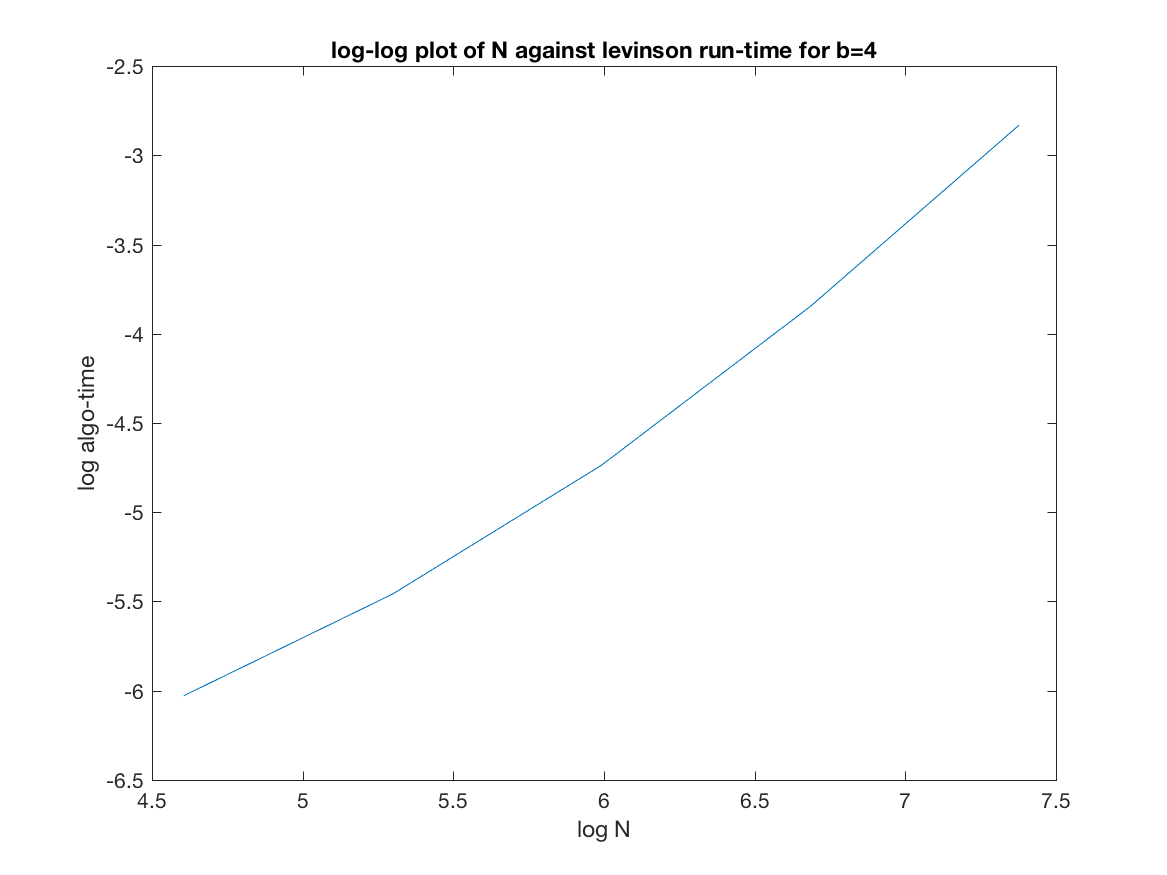
\includegraphics[width=0.8\textwidth]{log-log_plot_levinson.png}
  \caption{log-log plot of \texttt{levinson\_solve} against $N$}
  \label{fig:Levplot}
\end{figure}

\noindent The difference in scale of the log-run-time compared to the \texttt{Force} and \texttt{fastForce} is enormous. Where we compared run time in the largest system of $\exp{6}$ to $exp{3}$, we now have run-time of merely $\exp{-3.2} \approx 0.05s$! This means that our exploitation of the system has been extremely successful. The full table of comparisons in run time is table \ref{table:2} below, as created by \texttt{timeCompare}


\begin{table}
\begin{center}
  \begin{tabular}{ c||c|c|c|c|c }
	    &  N=100  &     N=200   &     N=400    &   N=800     &  N=1600 \\
    \hline

    Force   &  0.11309   &   0.43964   &    3.0571   &   40.561    &  390.05 \\
    fastForce     & 0.022626   &  0.082582   &   0.39377   &   2.8176    &  40.082 \\
    levinson      & 0.010291   & 0.0095507  &  0.0099089   & 0.023583   & 0.058483 \\

  \end{tabular}
\end{center}
\caption{Estimated Speed-up for Different Algorithms with Varying $N$}
\label{table:2}
\end{table}

Also created by this script is the speed-up table, which divides run-times to give an impression of how much quicker one algorithm performs than another.\\

\begin{table}
\begin{center}
  \begin{tabular}{ c||c|c|c|c|c }
	
            &       N=100   &  N=200  &   N=400 &   N=800  &   N=1600\\
	\hline

    Force/fastF   &    4.998  &  5.3237  &  7.7638 &   14.396 &   9.7315\\
    fastF/levin  &  2.1986  &  8.6467  &  39.739  &  119.47  &  685.36\\
    Force/levin    &  10.989  &  46.032  &  308.53  &  1719.9  &  6669.6
  \end{tabular}
\end{center}
\caption{Run-time for Different Algorithms with Varying $N$}
\label{table:3}
\end{table}

\noindent The last thing \texttt{timeCompare} produces is a log-log plot of the run-time of all algorithms in one place, to visualise the above data, seen in plot \ref{fig:timeCompare}.\\

\begin{figure}[h!]
  \centering
  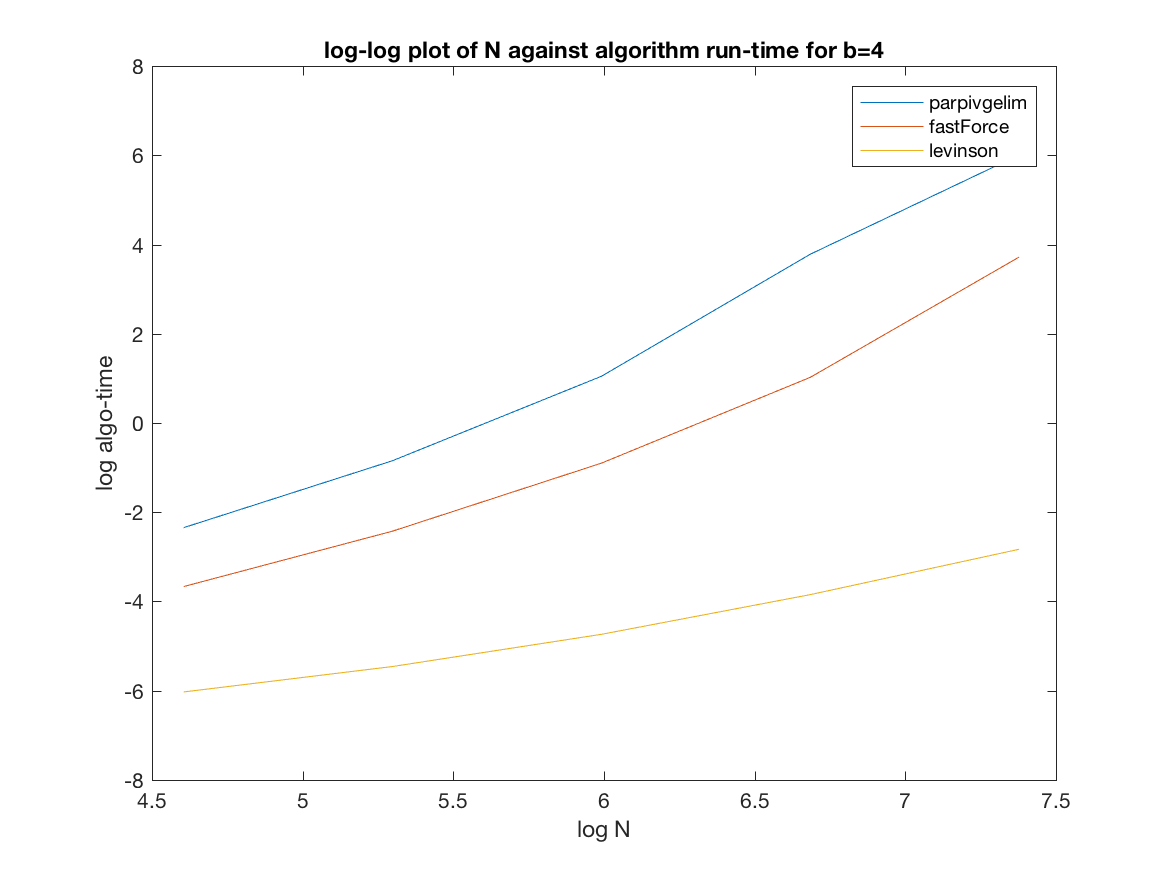
\includegraphics[width=0.8\textwidth]{log-log_plot_timecomparison.png}
  \caption{log-log plot comparing algorithm run-time against $N$}
  \label{fig:timeCompare}
\end{figure}


\\
\noindent So we can see that in the most extreme case, full exploitation of the matrix structure in the linear system allowed for almost a $7000\times$ speed up from the original case, which is incredible and demonstrates the power of exploiting matrix structure in linear systems.  


\newpage








\addcontentsline{toc}{section}{Appendix}
\newpage
\begin{appendix}
\listoffigures
\listoftables

\end{appendix}
\addcontentsline{toc}{section}{References}
\begin{thebibliography}{1}
 \bibitem{1}
 Golub \& Van Loan, ``Matrix Computations'' (2012) Chapter 4. \\
\end{thebibliography}

\end{document}







